\section{Diseño de la Solución}

Este sistema de gestión de inventarios fue diseñado bajo una arquitectura web full-stack, separando claramente la interfaz de usuario (frontend), la API (backend), y la persistencia de datos (base de datos).

\subsection{Componentes}

El sistema se compone de tres componentes principales:

\begin{itemize}
    \item \textbf{Frontend}: Aplicación desarrollada en React, responsable de la interacción con el usuario, validación de formularios y consumo de la API REST.
    \item \textbf{Backend}: API REST construida con Java Spring Boot, encargada de la lógica, autenticación, autorización y comunicación con la base de datos.
    \item \textbf{Base de Datos}: Servidor MySQL que almacena la información de usuarios, productos, inventario y operaciones.
\end{itemize}

\subsection{Interacción entre Componentes}

\begin{itemize}
    \item El usuario accede a la aplicación web desde su navegador y realiza acciones como iniciar sesión, registrar productos o consultar el inventario.
    \item El frontend envía solicitudes HTTP a la API REST del backend, que valida y procesa las peticiones.
    \item El backend interactúa con la base de datos MySQL para almacenar o recuperar información según la operación solicitada.
    \item Las respuestas del backend son procesadas por el frontend, que actualiza la interfaz de usuario en tiempo real.
    \item Para ciertas operaciones, el usuario puede exportar la información visualizada en la interfaz a un archivo PDF.
\end{itemize}

% 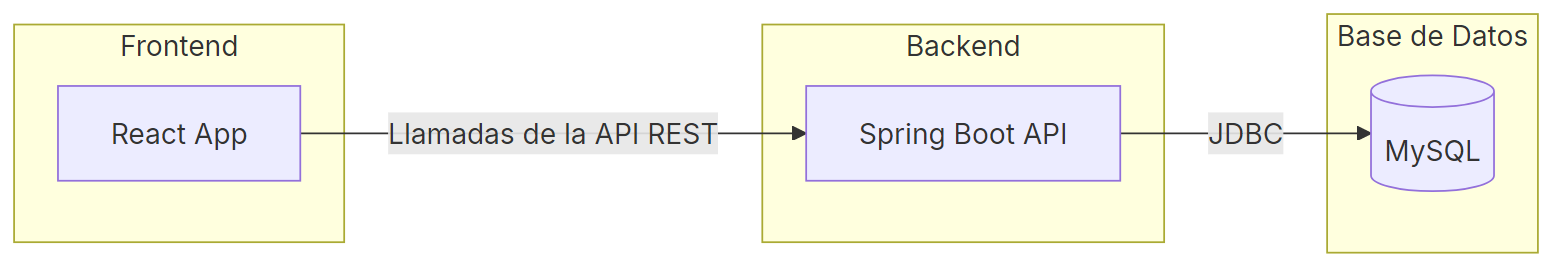
\includegraphics{diagrams/architecture.png}

\subsection{Casos de Uso}

El sistema tiene los siguientes casos de uso principales:

\begin{itemize}
    \item Registro y autenticación de usuarios.
    \item Alta, baja, modificación y consulta de productos en el inventario.
    \item Exportación de reportes en PDF.
\end{itemize}

El sistema implementa autenticación basada en JWT (JSON Web Tokens) para proteger los endpoints sensibles y garantizar que solo los usuarios autorizados puedan realizar operaciones sobre el inventario.

A continuación, los diagramas para los distintos casos de uso:

% \includegraphics{diagrams/todos los de caso de uso}

\subsection{Modelo de Datos}

La base de datos relacional está compuesta por las siguientes tablas principales:

\begin{itemize}
    \item \textbf{users}: Almacena la información de los usuarios registrados, incluyendo credenciales.
    \item \textbf{items}: Contiene los datos de los productos disponibles, incluyendo nombre, descripción, precio y cantidad.
    \item \textbf{operations}: Guarda un historial de las operaciones realizadas sobre el inventario.
\end{itemize}

% 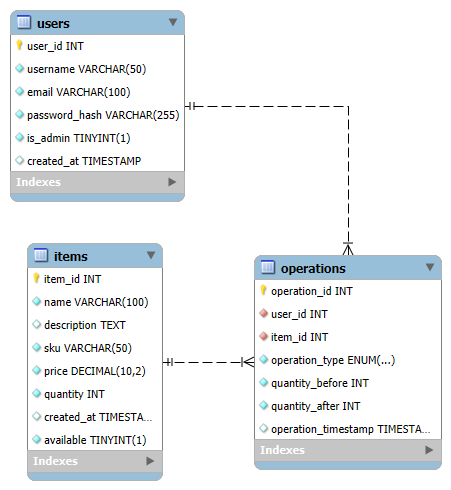
\includegraphics{diagrams/inventorydb.png}
